%author : berenice delcroix-oger

\documentclass[border=2pt]{standalone}
\usepackage{tikz}
\usetikzlibrary{positioning, fit, shapes, arrows, calc}

\pgfdeclarelayer{bg}    % declare background layer
\pgfsetlayers{bg,main}  % set the order of the layers (main is the standard layer)

\newcommand{\coula}{0785F2}
\newcommand{\coulb}{F29F05}
\newcommand{\coulc}{F21313}
\newcommand{\could}{E6F21F}



\definecolor{part1}{HTML}{\coula}
\definecolor{part2}{HTML}{\coulb}
\definecolor{part3}{HTML}{\coulc}
\definecolor{part4}{HTML}{\could}

\begin{document}
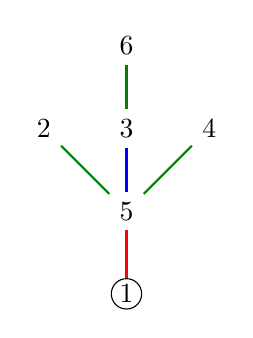
\begin{tikzpicture}[scale=0.7, grow=up]
\node[draw, circle, inner sep=1pt] {1}
   child[red, thick]{node[black]{5}
      child[green!50!black]{node[black]{4}}   
      child[blue]{node[black]{3}
          child[green!50!black]{node[black]{6}}         
      }   
      child[green!50!black]{node[black]{2}}   
   };
\end{tikzpicture}

\end{document}
